Gravitational waves are 'ripples' in space-time caused by some of the most violent and energetic processes in the Universe. Albert Einstein predicted the existence of gravitational waves in 1916 in his general theory of relativity. Einstein's mathematics showed that massive accelerating objects (things like neutron stars or black holes orbiting each other) would disrupt space-time in such a way that 'waves' of undulating space-time would propagate in all directions away from the source. These cosmic ripples would travel at the speed of light, carrying with them information about their origins, as well as clues to the nature of gravity itself.\\

Observations revealed that the orbit of this binary star system was decaying at a rate predicted (to near-perfect precision) by the radiation of gravitational waves due to the orbital motion of the neutron stars. Forty-two years after this initial evidence of their existence, the first direct detection of gravitational waves was announced by the LIGO Virgo Collaborations in 2016.\\

The history of gravitational waves over the century preceding this discovery was at times controversial: from Einstein’s attempt in 1937 to overturn his initial 1916 prediction of their existence; to pioneering, albeit premature, claims of detection by Weber in the 1960s. Seven years on from this historic first discovery, nearly 100 gravitational wave events have been observed, all from colliding binary systems of pairs of black holes (including the first discovery), pairs of neutron stars, or a black hole and a neutron star.\\

\begin{figure}[h]
\centering
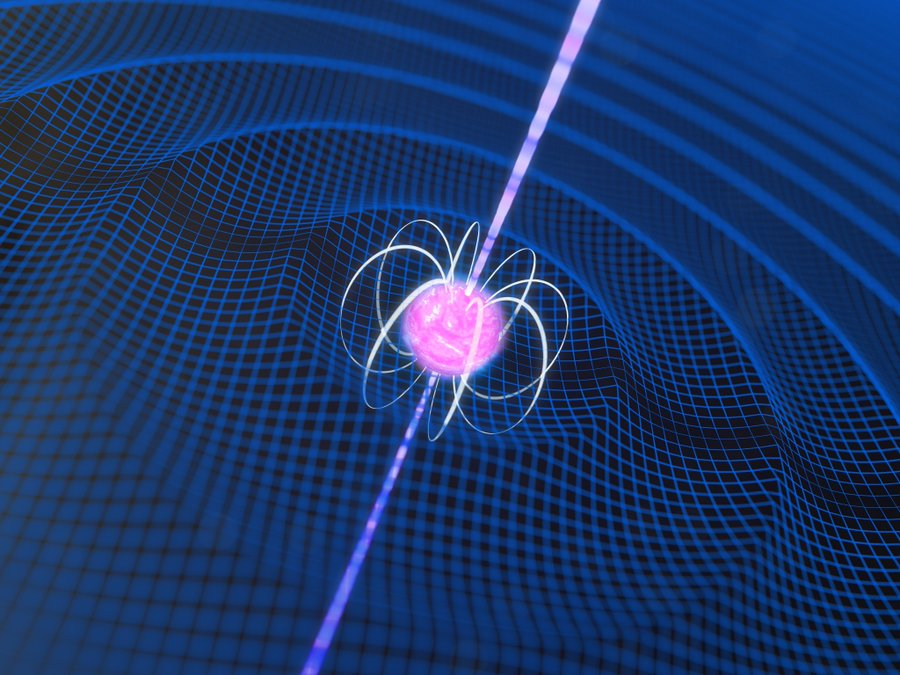
\includegraphics[height=0.4\textwidth, width=0.5\textwidth]{images/Continous gravitational wave.jpg}
\caption{\small Artist’s impression of a neutron star radiating both continuous gravitational waves and electromagnetic radiation. Credit: OzGrav/Carl Knox.}
\end{figure}

\begin{figure}[h!]
\centering
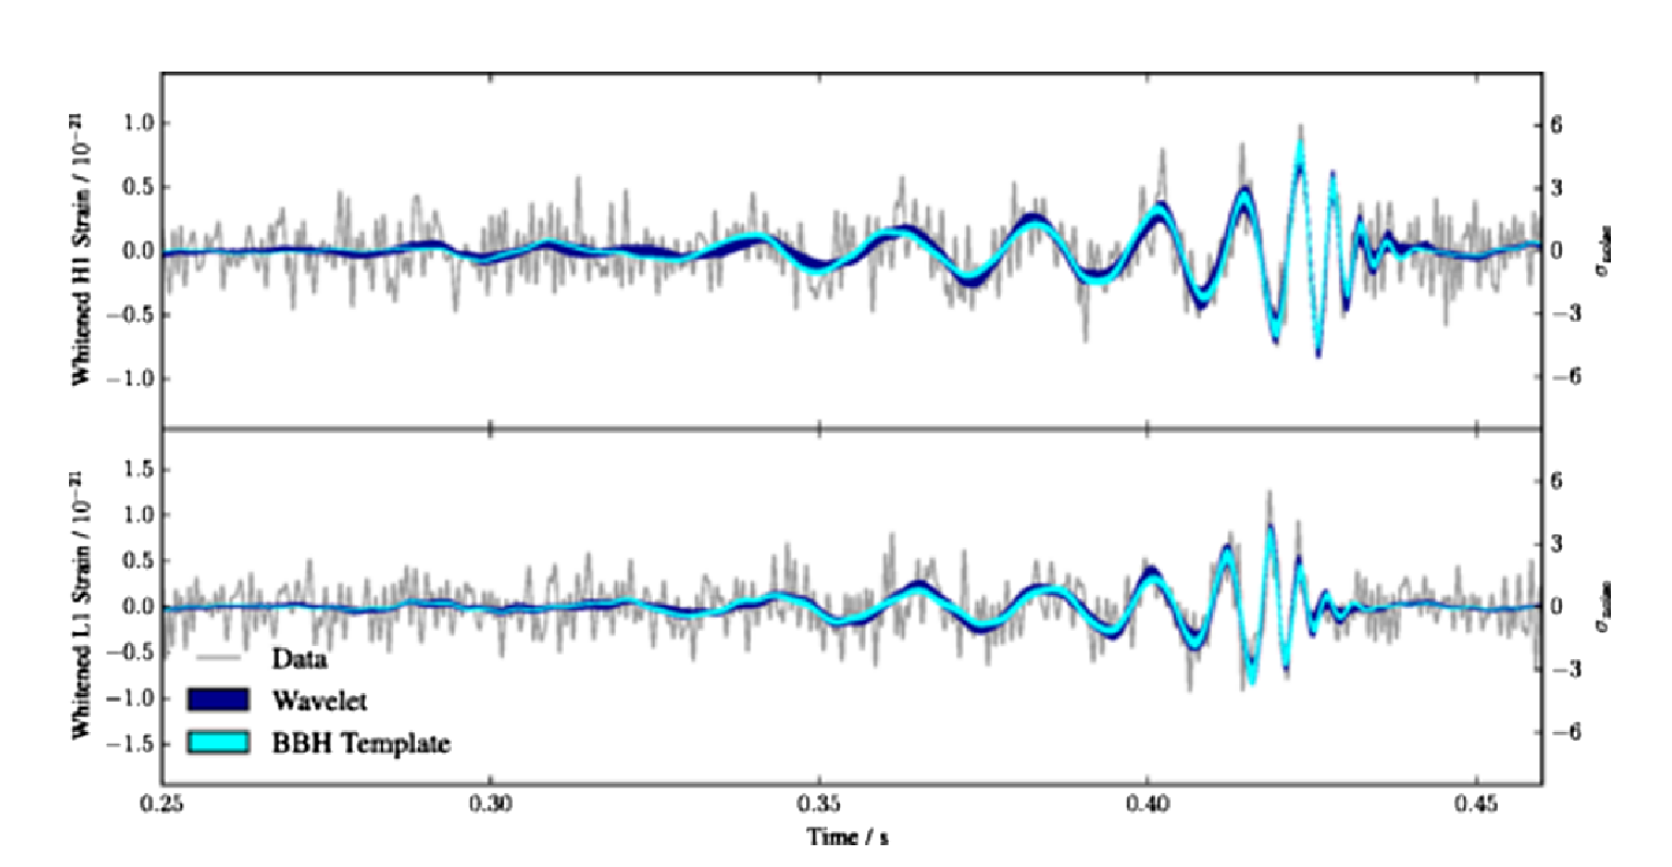
\includegraphics[height=0.7\textwidth, width=0.7\textwidth]{images/mass_estimation_graph.png}
\caption{\small Measured detector strain time series of the first detected gravitational wave signal by Advanced LIGO, GW150914 (B. P. Abbott et al., 2016b) as observed in H1 (top panel) and L1 (bottom panel).}
\end{figure}

Gravitational wave observations may, however, be able to detect neutron stars which are deformed from spherical symmetry. A number of mechanisms, including a strong magnetic field permeating the star, accretion of matter from a companion star, or periodic oscillations akin to travelling Rossby waves in the Earth’s oceans, could perturb the neutron star away from axis symmetry about its rotation axis. General relativity predicts that the neutron star would then radiate a continuous stream of gravitational waves at twice its rotational frequency; these are known as continuous gravitational waves. Beyond signal detection, a major challenge has been the development of statistical and computational methodology for estimating the physical waveform parameters.\citeauthorandyear{param_estim}\\

The physical parameters estimated for this signal include the masses, spins, luminosity distance, sky position, and other parameters. Using parameter estimation the initial component masses of the system in the source frame was found corresponding to GW150914. Some of the types of parameter estimation are:

\begin{itemize}
    \item Markov Chain Monte Carlo
    \item Nested Sampling
    \item Model Comparison
    \item Rapid Parameter Estimation
    \item Machine Learning
\end{itemize}

We are becoming more sensitive to gravitational waves. The second-generation gravitational wave detectors that are currently in use are undergoing upgrades, and it is projected that soon these detectors will start running nearly continuously, greatly expanding the amount of data that is available for study. An order of magnitude increase in sensitivity is anticipated for the third generation of ground-based gravitational wave detectors, which are slated to start construction in the 2030s.\\

Once they are discovered, continuous gravitational waves will offer an astronomical instrument unlike any other for studying the physics of neutron stars. Continuous gravitational waves, which result from asymmetric mass distributions within the star but originate from the exterior of the star like electro-magnetic emission from neutron stars, are more sensitive to the physics of the star's interior. Additionally, continuous gravity waves would continuously explore the non-symmetric condition of deformed neutron stars over long periods of time, in contrast to electromagnetic observations that infer macroscopic features of spherically symmetric neutron stars and binary neutron star merger signals that persist just a short time. Therefore, it is crucial that data processing techniques are developed that can extract the physical information sent by continuous gravitational waves in advance of a first discovery.\\

Based on observed rates of Supernovae, it is estimated that there may be up to a billion neutron stars in the Milky Way, only a few thousand of which are currently observed as pulsar. \citeauthorandyear{Sartore2010} Constant gravitational waves present a rare chance to see neutron stars that cannot be detected as pulsars and are therefore invisible to electromagnetic observatories. It is necessary to build templates that span the range of potential parameters because the template waveform parameters of these neutron stars are unknown. One would expect the neutron star to spin more slowly as its rotational energy is radiated away in gravitational waves, similar to the loss of orbital energy from the Hulse-Taylor binary pulsar, as well as the position of the neutron star in the sky and the evolution of gravitational wave frequency over time. Unfortunately, this parameter space quickly becomes vast, particularly given that the continuous gravitational wave signals must be traced over a year or more of detector data. The time taken to analyse the data, even on modern computing hardware, quickly becomes prohibitive, and one must instead adopt suboptimal data analysis strategies which are less costly.\\

\newpage

\subsection{Gravitational Wave Analysis of Magnetars}

Newly born magnetars are expected to emit long lasting GW transients in the first hours after their birth.  Such GW signals can be much stronger than that from the core collapse itself and therefore detectable up to larger distances. Thus, even though magnetars occur only in 10 of Core Collapse Supernovae (CCSNe), they can be detected in GWs with a larger event rate if the search horizon is greater than 2 3 times that of CCSNe.\\


\begin{figure}[h]
\centering
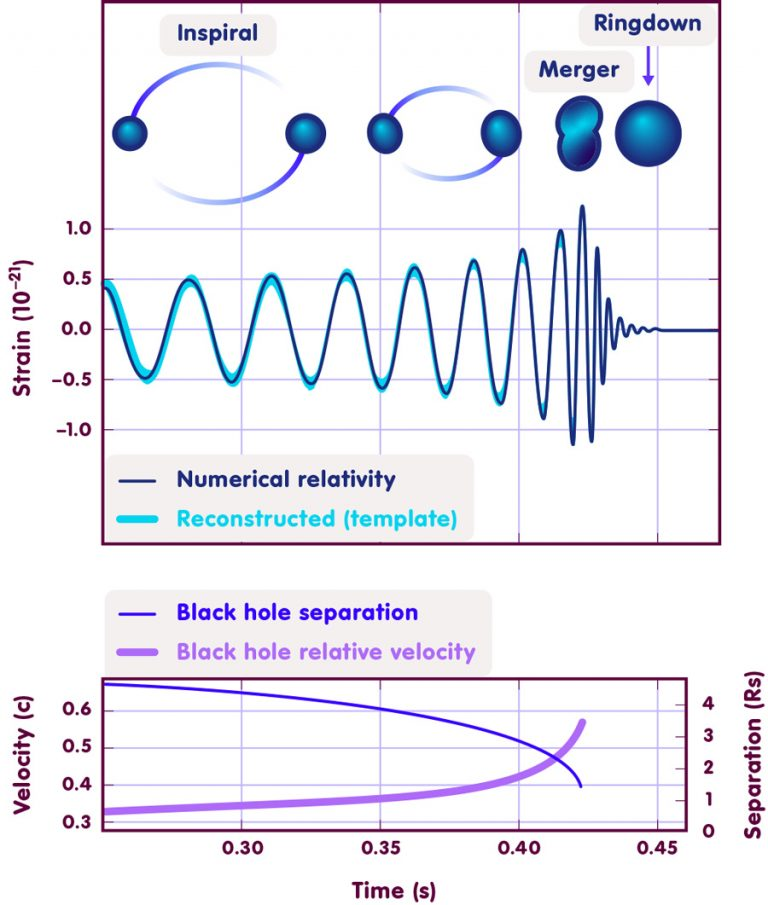
\includegraphics[height=0.8\textwidth, width=0.7\textwidth]{images/grav_wave_graph.jpg}
\caption{\small Estimated gravitational wave amplitude of GW150914 at the Hanford detector. Above that are the Schwarzschild horizons of both merging black holes shown as calculated numerically from the general theory of relativity. Below: The effective distance of the black holes in units of Schwarzschild radii RS and the relative velocity in units of the speed of light. [Image: LIGO / Redesign: Daniela Leitner]}
\end{figure}

Magnetar-driven shock breakouts (SBOs) can provide crucial electromagnetic (EM) triggers for GW searches of long-transients emitted by newly formed magnetars. They will help enhance the sensitivity of GW searches in two complementary ways: on the one hand by providing the start time for the transient signal, and on the other hand by constraining the NS spin period and B-field, which in turn determine the GW signal shape.\\

Magnetar-driven SBOs detected by ULTRASAT will have for the joint search of GW long transients emitted by newly born magnetars. Not only will magnetardriven SBOs represent a necessary EM trigger for GW searches, but they will also provide direct constraints on the GW signal parameters. Both factors will contribute to improving the sensitivity of GW searches, hence extending their horizon and the expected event rate (0.1  $ yr^{-1}$).\citeauthorandyear{Magnetar_GW}\\

